	\documentclass[10pt,oneside]{CBFT_book}
	% Algunos paquetes
	\usepackage{amssymb}
	\usepackage{amsmath}
	\usepackage{graphicx}
% 	\usepackage{libertine}
% 	\usepackage[bold-style=TeX]{unicode-math}
	\usepackage{lipsum}

	\usepackage{natbib}
	\setcitestyle{square}

	\usepackage{polyglossia}
	\setdefaultlanguage{spanish}
	



	\usepackage{CBFT.estilo} % Cargo la hoja de estilo

	% Tipografías
	% \setromanfont[Mapping=tex-text]{Linux Libertine O}
	% \setsansfont[Mapping=tex-text]{DejaVu Sans}
	% \setmonofont[Mapping=tex-text]{DejaVu Sans Mono}

	%===================================================================
	%	DOCUMENTO PROPIAMENTE DICHO
	%===================================================================

\begin{document}




% =================================================================================================
\chapter{Picture de interacción y perturbación dependiente del tiempo}
% =================================================================================================

Estudiaremos perturbaciones dependientes del tiempo 
\[
	H = H_0 + V(t), \qquad H_0 \Ket{n} = E_n \Ket{n}
\]
donde, no obstante, $\Ket{n}$ no dependiente del tiempo. 
La idea es que hasta $t=0$ no hay potencial $V$ y luego al {\it encenderse} el potencial el estado pasará
a otro
\[
	\Ket{i} \longrightarrow \Ket{j}.
\]

Se estudiarán transiciones entre autoestados del mismo hamiltoniano $H_0$ (que son estacionarios). 
Un autoestado permanece en el tiempo como tal pero con fase oscilante (como veremos).
\notamargen{Esta deduccióne está diferente de la carpeta, confío en que sea una versión depurada.
Se la analizará en la próxima fase.}
\[
	\Ket{\alpha,t_0,t}_s = \euler^{-iH/\hbar(t-t_0)}\Ket{\alpha,t_0}_s
\]
\[
	= \euler^{-iH/\hbar(t-t_0)} \euler^{-iV(t)/\hbar(t-t_0)} \Ket{\alpha,t_0}
\]
\[
	= \sum_n \euler^{-iH_0/\hbar \: t} \euler^{-iV(t)/\hbar \: t} \ket{n}\Braket{n|\alpha,t_0}
\]
\[
	= \sum_n \euler^{-iE_n^0/\hbar \: t }\ket{n}\euler^{-iV(t)/\hbar \: t } \Braket{n|\alpha,t_0}	
\]
\[
	\euler^{iH_0/\hbar t}\Ket{\alpha,t_0,t}_s =
	\sum_n  \underbrace{\euler^{-iV(t)/\hbar \: t} \Braket{n|\alpha,t_0}}_{C_n(t)} \ket{n} = \Ket{\alpha,t_0,t}_I	
\]
es decir que se escriben los kets como
\[
	 \Ket{\alpha,t_0,t}_I = \euler^{iH_0/\hbar t}\Ket{\alpha,t_0,t}_s.
\]
Aquí se puede pensar que 
\begin{itemize}
 \item $C_n(t)$ evoluciona por $V(t)$
 \item $\euler^{-iE_n^0 t/\hbar}$ evoluciona por $H_0$
\end{itemize}

Esto introduce la {\it picture} (o representación) de Dirac, también llamada ``de interacción'', en la 
cual los estados evolucionan con $V(t)$.
La siguiente tabla compara con las anteriores [atrasarla porque lo de los operadores aparece después]
\begin{center}
\begin{tabular}{|c|ccc|}
\hline 
& Dirac & Schrödinger & Heinsenberg \\
\hline 
% & &  & \\
estados & evolucionan & evolucionan & fijos \\
$\Ket{\alpha}$ & con $V(t)$ & con $H$ &  \\
\hline
operadores & evolucionan & fijos & evolucionan \\
 & con $H_0$ &  & con $H$ \\
\hline
base & fijos & fijos & evolucionan \\
$\Ket{a'}$ &  &  &  \\
\hline 
% & & & \\
\end{tabular}
\end{center}

\[
	i\hbar \dpar{}{t}\Ket{\alpha,t_0,t}_s = H \Ket{\alpha,t_0,t}_s
\]
\[
	i\hbar \dpar{}{t}\left( \euler^{-iH_0t/\hbar}\Ket{\alpha,t_0,t}_I \right) = 
	H \euler^{-iH_0t/\hbar} \Ket{\alpha,t_0,t}_I
\]
\[
	i\hbar \euler^{-iH_0t/\hbar}\dpar{}{t} \Ket{\alpha,t_0,t}_I = 
	V(t) \euler^{-iH_0t/\hbar} \Ket{\alpha,t_0,t}_I
\]
\[
	i\hbar \dpar{}{t} \Ket{\alpha,t_0,t}_I = V(t) \Ket{\alpha,t_0,t}_I,
\]
que es la ecuación de evolución de los kets, y es equivalente a la ecuación de Schrödinger.

La definición debe verificar asimismo que 
\[
	_s\Braket{\; A_s \;}_s = _I\Braket{\; A_I \;}_I,
\]
lo cual conduce a
\begin{multline*}
	_I\Braket{\alpha,t_0,t|A_I|\alpha,t_0,t}_I = \\
	_s\Braket{\alpha,t_0,t|\euler^{-iH_0t/\hbar}A_I\euler^{iH_0t/\hbar}|\alpha,t_0,t}_s = 
	_s\Braket{\alpha,t_0,t|A_s|\alpha,t_0,t}_s,
\end{multline*}
o bien a que los operadores evolucionan según 
\[
	A_I = \euler^{iH_0t/\hbar}A_s\euler^{-iH_0t/\hbar}
\]
\[
	\dtot{A_I}{t} = \frac{1}{i\hbar}[A_I, H_0]
\]
que es igual que la ecuación de Heisenberg pero con $\hat{H}_0$ en lugar de $H$.
Los kets base permanecen fijos, porque así lo hacen en Schrödinger, en realidad oscila su fase; entonces 
\[
	\Ket{n,t_0,t}_s = \euler^{-iHt/\hbar} \ket{n,t_0}_s
\]
\[
	\Ket{n,t_0,t}_I = \euler^{iH_0t/\hbar} \euler^{-iHt/\hbar} \ket{n,t_0}_s =
	\euler^{-iVt/\hbar} \ket{n,t_0}_s = \euler^{iH_0t/\hbar} \ket{n,t_0}_s
\]
\[
	\Ket{n,t_0,t}_I = \euler^{iE_0t/\hbar} \ket{n,t_0,t}_s
\]
\notamargen{En la carpeta está primero lo de los kets base y luego la ecuación de movimiento 
que acá aparece inmediatamente debajo de la tabla. Aquí habrá que reordenar material.}

Finalmente, resta ver qué le sucede a los coeficientes.

\[
	\Ket{\alpha,t_0,t}_I = \sum_n \Ket{n}\Braket{n|\alpha,t_0,t}_I = \sum_n C_n(t) \Ket{n}
\]
\[
	C_n(t) = \euler^{iVt/\hbar} \Braket{n|\alpha,t_0}_s
\]
\[
	\Braket{n|\alpha,t_0,t}_I = C_m(t)
\]
con $\Ket{n},\ket{m}$ autoestados de $H_0$, le pego un $\Bra{n}$ a la ecuación de evolución de kets,
\[
	i\hbar \dpar{}{t} \Braket{n|\alpha,t_0,t}_I = \Braket{n|V_I(t)|\alpha,t_0,t}_I
\]
\[
	= \sum_m \Braket{n|V_I(t)|m}\Braket{m|\alpha,t_0,t}_I
\]
\[
	i\hbar \dpar{}{t}C_n(t) = \sum_m C_m(t) \Braket{n|V_I(t)|m}
\]
\[
	i\hbar \dpar{}{t}C_n(t) = \sum_m C_m(t) \Braket{n|V_s|m} \euler^{it(E_n-E_m)/\hbar}
\]
\[
	i\hbar \dpar{}{t}C_n(t) = \sum_m C_m(t) V_{nm}(t) \euler^{i\omega_{nm}t}
\]
donde $V_{nm}(t) \equiv \Braket{n|V(t)|m}$ y $\omega_{nm} \equiv (E_n-E_m)/\hbar$.
Esta es la ecuación que cumplen los coeficientes, donde $|C_n(t)|^2$ es la probabilidad de hallar al sistema 
en el autoestado $\Ket{n}$.
Resolver esto puede ser muy difícil, salvo en los casos en que es tan fácil que no nos
sirve de nada \footnote{Esto es un patrón que se observa a menudo en física teórica.}.
Esto puede ponerse en forma matricial como
\[
	i\hbar \begin{pmatrix}
	\dot{c}_1 \\ \dot{c}_2 \\ ... \\ \dot{c}_N \\
	\end{pmatrix} 
	=
	\begin{pmatrix}
	V_{11} & V_{12}\euler^{i\omega_{12}} & ... \\ 
	V_{21}\euler^{i\omega_{21}} & V_{22} & ... \\ 
	... \\ 
	... \\
	\end{pmatrix}
	\begin{pmatrix}
	c_1 \\ c_2 \\ ... \\ c_N \\
	\end{pmatrix} .
\]


\subsection{Método perturbativo (dependiente del tiempo)}

Pensaremos en una serie perturbativa 
\[
	C_n(t) = C_n(t)^{(0)} + C_n(t)^{(1)}  + C_n(t)^{(2)}  + ...
\]

El evolucionador temporal en la picture de interacción cumple 
\[
	\Ket{\alpha,t_0,t} = U_I(t,t_0)\Ket{\alpha,t_0}_I, \qquad t > t_0
\]
que viene de  
\[
	i\hbar \dtot{}{t} U_I(t,t_0) = V_I(t) U_I(t,t_0)
\]
con $U_I(t_0,t_0)=\mathbb{1}$, la cual resolviendo nos hace llegar a 
\[
	U_I(t,t_0) = \mathbb{1} - \frac{i}{\hbar}\int_{t_0}^{t} V_I(t')U_I(t',t_0) dt'.
\]

Esta ecuación debe proporcionarnos la forma de hallar $U_I$. Se puede usar una iteración sencilla
\[
	U_I(t,t_0) = \mathbb{1} - \frac{i}{\hbar} \int_{t_0}^t \: V_I(t') \left[ 
	\mathbb{1} - \frac{i}{\hbar} \int_{t_0}^t \: V_I(t'') U_I(t'',t_0) dt''
	\right] \: dt',
\]
\[
	U_I(t,t_0) = \mathbb{1} - \frac{i}{\hbar} \int_{t_0}^t \: V_I(t') \left[ 
	\mathbb{1} - \frac{i}{\hbar} \int_{t_0}^t \: V_I(t'') \left(
	\mathbb{1} - \frac{i}{\hbar} \int_{t_0}^t \: V_I(t''') \left\{ ... \right\} dt''
	\right) dt''
	\right] \: dt',
\]
y esto lleva a la serie de Dyson, casi una expresión formal,
\begin{multline*}
	U_I(t,t_0) = \mathbb{1} - \frac{i}{\hbar}\int V_I(t') dt' + \left( -\frac{i}{\hbar} \right)^2\int_{t_0}^t 
	V_I(t') \int_{t_0}^{t'}V_I(t'')dt'' + ...\\ + \left( -\frac{i}{\hbar} \right)^n 
	\int_{t_0}^t dt'\int_{t_0}^{t'}dt''\int_{t_0}^{t''}dt''' ... \int_{t_0}^{t^{n-1}}dt^{n} V_I(t') 
	V_I(t'')...V_I(t^n)	
\end{multline*}
que es una especie de exponencial $ \euler^{T[-i/\hbar \int V(t) dt ]}$.

La serie de Dyson puede verse como un desarrollo perturbativo.

\subsection{Transiciones entre autoestados del hamiltoniano $H_0$}

Veamos el detalle de las transiciones en el formalismo de Dirac.
\[
	\Ket{i,t_0=0,t}_I = U_I(t,0) \Ket{i} = \sum_n \Ket{n}\Braket{n|U_I(t)|i}
\]
y como se viera oportunamente
\[
	\Ket{i,t}_I = \sum_n C_n(t)\Ket{n} = \sum_n \left( \Braket{n|U_I(t)|i} \right) \Ket{n}.
\]
La amplitud de transición será 
\[
	C_n(t) = \Braket{n|U_I(t)|i}
\]
con $\Ket{i},\Ket{n}$ autoestados de $H_0$.
Sea $\tilde{C}_n(t)=\Braket{n|U_s(t)|i}$, donde vemos que $\tilde{C}_n(t)$ y $C_n(t)$ difieren en
una fase, y busquemos una expresión 
\[
	\Ket{\alpha, t_0, t}_I = \euler^{iH_0t/\hbar} \Ket{\alpha, t_0, t}_s
\]
\[ 
	= \euler^{iH_0t/\hbar} U_S(t,t_0)\Ket{\alpha, t_0}_s
\]
\[
	\Ket{\alpha, t_0, t}_I  = \euler^{iH_0t/\hbar} U_S(t,t_0) \euler^{-iH_0t_0/\hbar}  \Ket{\alpha, t_0}_I
	= U_I(t,t_0) \Ket{\alpha,t_0}_I
\]
\[
	\euler^{iH_0t/\hbar} \hat{U}_S \euler^{-iH_0t_0/\hbar} = \hat{U}_I
\]
y notemos que $\hat{U}$ no obedece la ley de transformación de operadores.

\[
	C_n(t) = \Braket{n|\euler^{iH_0t/\hbar} U_S(t,t_0) \euler^{-iH_0t_0/\hbar}|i}
\]
\[
	C_n(t) = \euler^{-i/\hbar[E_n^{(0)} t - E_i^{(0)} t_0]} \Braket{n| U_S(t,t_0) |i} =
		\euler^{-i/\hbar[E_n^{(0)} t - E_i^{(0)} t_0]} \tilde{C}_n(t)
\]
lo que lleva a 
\[
	|C_n(t)|^2 = |\tilde{C}_n(t)|^2.
\]
Para transiciones entre autoestados de $H_0$ los coeficientes dan la misma probabilidad 
(evaluados con el evolucionador de Dirac que con el de Schrödinger).
Debe notarse que esto se cumple siempre y cuando la transición sea entre autoestados del
hamiltoniano y la fase resulte así global.


Veamos las transiciones 
\[
	\Braket{ n | U_I(t,t_0)| i }
\]
a los diferentes órdenes en la perturbación
\begin{itemize}
 \item orden 0
 \[
	C_n^{(0)}(t) = \Braket{n|1|i} = \delta_{ni}
 \]
 \item orden 1
 \[
 	C_n^{(1)}(t) = -\frac{i}{\hbar} \int_{t_0}^t \euler^{i\omega_{ni} t'} V_{ni}(t') dt' \qquad \qquad 
 	V_{ni} \equiv \Braket{n|V(t)|i}
 \]
 \item orden 2
 \[
 	C_n^{(2)}(t) = \sum_m \left( -\frac{i}{\hbar} \right)^2  \int_{0}^t  dt'\int_{0}^t dt''
 	\euler^{it'/\hbar(E_n-E_m)} V_{nm}(t') \euler^{it''/\hbar(E_m-E_i)} V_{mi}(t'')
 \]
\end{itemize}
y entonces la probabilidad de ir desde $\ket{i} \to \Ket{n}$ con $i\neq n$, hasta orden dos, sería
\[
	P^{(2)}_{i\to n} = |C_n^{(0)}(t)+C_n^{(1)}(t)+C_n^{(2)}(t)|^2 =
	| C_n^{(1)}(t) + C_n^{(2)}(t) |^2
\]
donde debe notarse que hay interferencia entre los diversos términos.

\subsection{Ejemplo: potencial constante encendido abruptamente}

Sea un potencial que prendemos y apagamos luego, pero constante. Es decir
\[
	V(t) = \begin{cases}
	0 	& t < 0  \\
	V(r,p,s,L,...) & t \geq 0
	\end{cases}
\]
donde $V \neq V(t)$, pero puede depender de cualquier otra cosa. La figurilla más abajo
ilustra este {\it escalón}.

\includegraphics[width=0.45\textwidth]{images/teo2_22.pdf}

A orden cero no vemos cambio pues
\[
	C^0_n(t) = 0.
\]
A orden uno es 
\[
	C^1_n(t) = -\frac{i}{\hbar} \int_0^t \euler^{i/\hbar(E_n - E_i)t'} V_{ni} \: dt'=
	\frac{V_{ni}}{(E_n - E_i)}(1-\euler^{i\omega_{ni}t})
\]
donde debemos notar que si esto revienta porque $E_n \sim E_i$ entonces la teoría de
perturbaciones no puede usarse aquí.

Evaluando la probabilidad se tiene	
\[
	|C^1_n(t)|^2 = 
	\frac{4|V_{ni}|^2}{| E_n - E_i|^2}\sin^2\left(\frac{(E_n - E_i)t}{2\hbar}\right).
\]

	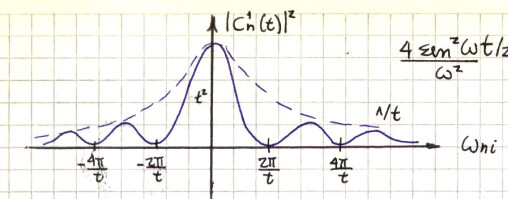
\includegraphics[width=0.45\textwidth]{images/fig_ft2_potencial_abrupto.jpg}

Es máxima la probabilidad cuando $\Delta E\to 0$. 
En ese caso las transiciones son a estados de la misma energía. 
El gráfico de arriba es a un dado $t$ fijo. A medida que el tiempo transcurre el gráfico
tiende a una delta de Dirac.

A tiempo largo la probabilidad es no nula para aquellos estados 
\[
	t \sim \frac{2\pi}{|\omega_{ni}|}
\]

Hay probababilidad de transición $\Ket{i} \to \Ket{n}$ apreciable donde $\omega = \frac{2\pi}{t}
= \frac{\Delta E}{\hbar}$ dado que $\Delta t \Delta E \sim \hbar $. O bien, $\Delta E \sim 0$.

\section{Scattering}

Podemos pensarlo como el caso de un potencial que se prende y apaga, representando éste el objeto
contra el cual se hace scattering.

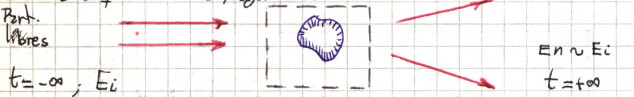
\includegraphics[width=0.6\textwidth]{images/fig_ft2_scattering_intro.jpg}

Este último ejemplo puede aplicarse a colisiones elásticas. Prendemos y apagamos un potencial que es el 
masacote al cual impactamos. De entrada ha partículas libres y de salida (lejos de $V$) partículas libres.
Entonces $ E_n - E_c \sim 0$ y consideraremos lo que sucede a tiempos largos. Interesará la probabilidad 
total de transicionear a estados de energía similares a $E_i$. Por ello se considera 
\be
	\sum_{\substack{n \\ E_n\sim E_i}} |C^1_n(t)|^2 
	\longrightarrow 
	\int \: \rho(E_n) \: |C^1_n(t)|^2 \: dE_n
	\label{scattering_integral}
\ee
donde el integrando es el número de estados dentro de un intervalo de energías $(E,E+dE)$ a los cuales
se puede transicionar. Esta erá la probabilidad de transición.

\begin{figure}[htb]
	\begin{center}
	\includegraphics[width=0.6\textwidth]{images/teo2_23.pdf}
	\end{center}
	\caption{}
\end{figure} 

A primer orden la probabilidad será algo como
\[
	\lim_{t\to\infty} \; \int \: \rho(E_n) \: \frac{4|V_{ni}|^2}{| E_n - E_i|^2}
	\sin^2\left(\frac{(E_n - E_i)t}{2\hbar}\right) \: dE_n,
\]
puesto que estamos considerando lo que sucede a tiempos muy largos.
En esos casos, como la probabilidad tiende a una delta de Dirac, 
\[
	\lim_{t\to\infty} \frac{1}{| E_n - E_i|^2}
	\sin^2\left(\frac{(E_n - E_i)t}{2\hbar}\right) = \frac{\pi t}{2\hbar} \delta(E_n - E_i),
\]
la integración es fácil y se obtiene
\[
	\lim_{t\to\infty} \; \int \: \rho(E_n) |C^1_n(t)|^2 \: dE = 
	\left.\left(\frac{2\pi}{\hbar}\right) \rho(E_n) |\bar{V}_{ni}|^2 \: t \: \right|_{E_n\sim E_i}
\]
donde $\bar{V}_{ni}$ es un potencial promedio. La probabilidad de transición es proporcional a $t$. 

Se suele definir una tasa de transición (probabilidad de transición por unidad de tiempo)
\[
	\dtot{}{t}\left( \sum_{\substack{n \\ E_n\sim E_i}} |C_n^{(1)}|^2 \right) =
	\left(\frac{2\pi}{\hbar}\right)	|\bar{V}_{ni}|^2 \rho(E_n) = \omega_{i\to n}^{(1)}
\]
que es la regla de oro de Fermi, y sirve para calcular cualquier transición entre estados
para potenciales que no dependen del tiempo.

[reacomodar]
La energía al final se mide con cierto error $\Delta E$ de modo que se obtendrá $E \pm \Delta E$ y 
deberá sumar [no sé bien qué se quiere decir acá]
\[
	\sum_n | C_n(t) |^2 \quad (E_n \sim E \pm \Delta E)
\]
Pero si no es discreto necesitaré integrar (la integral \eqref{scattering_integral})

\section{El método variacional}

Se puede usar para aproximar la energía del estado fundamental (el estado de energía mínima).
No conocemos $\Ket{n}$ ni $E_n$, pero $ H \Ket{n} = E_n \Ket{n}$ donde $\{ \Ket{n} \}$ es
una base.
Evaluamos
\[
	\Braket{\psi|H|\psi} = \sum_{n,m}\Braket{\psi|n}\Braket{n|H|m}\Braket{m|\psi} =
		\sum_{n,m} E_n \Braket{\psi|n}\Braket{n|m}\Braket{m|\psi} 
\]
\[
	\Braket{\psi|H|\psi} = \sum_{n,m} E_n C_n^*\Braket{n|m}C_m = \sum_{n} E_n|C_n|^2
\]
\[
	\sum_{n} E_n|C_n|^2 \geq \sum_n E_0|C_n|^2 = E_0 \sum_n |C_n|^2 = E_0 \Braket{\psi_n|\psi_n}
\]
y usamos 
\[
\Ket{\psi} = \sum_n \Braket{n|\psi}\Ket{n} \qquad \Bra{\psi} = \sum_n \Braket{\psi|n}\Bra{n} 
\]
para arribar a
\[
	\frac{\Braket{\psi_n|H|\psi_n}}{\Braket{\psi_n|\psi_n}} \geq E_0.
\]
donde $E_0$ es la energía más baja. Esto no parece ser muy iluminador que digamos.
Se considera que $\psi$ es tal que 
\[
	\Braket{x|\psi} = \psi(x)_{|x|\to\infty} \to 0
\]
lo que significa que la función de onda es {\it well behaved} (bien comportada).

\begin{ejemplo}{\bf Ejercicio 10}

A partir de $ \Braket{x|\psi} = \euler^{-\b|x|}$ se tiene, intercalando la completitud,
\[
	\Braket{\psi|\psi} = 
	\int_{-\infty}^\infty \: \Braket{\psi | x'}\Braket{x' | \psi} \: dx' = 
	2 \int_{-\infty}^\infty \: \euler^{- 2 \b |x| } \: dx = \frac{1}{\b}
\]
y del mismo modo
\begin{multline*}
	\Braket{\psi|H|\psi} = \Braket{\psi| \frac{p^2}{2 m} + \frac{m \omega^2 x^2 }{2} |\psi} = \\
	- \Frac{\hbar^2}{2m} \int_{-\infty}^\infty \: 
	\dtot[2]{}{x}\left( \Braket{\psi|x} \right)\Braket{x'|\psi} \: dx' +
	\frac{m\omega^2}{2} \int_{-\infty}^\infty \: \Braket{\psi|x^2|x'} \Braket{x'|\psi} \: dx',
\end{multline*}
para finalmente
\[
	\Braket{\psi|H|\psi} = - \Frac{\hbar^2}{2m} \int_{-\infty}^\infty \: 
	\dtot[2]{}{x}\left( \euler^{- \b |x| } \right) \euler^{- \b |x| } \: dx' +
	\frac{m\omega^2}{2} \int_{-\infty}^\infty \: \euler^{- 2 \b |x| } x^2 \: dx'
\]

Trabajaremos por partes esta cosa. Una integral con la doble derivada se convierte en
\[
	\int_{-\infty}^\infty \: u \dtot[2]{u}{x} \: dx = 
	\left. u \: \dtot{u}{x} \right|_{-\infty}^\infty - \int_{-\infty}^\infty \: \Dtot{u}{x}^2 \: dx
\]
donde el primer término es nulo porque la función de onda es bien comportada.
Con este enfoque resulta
\[
	\Braket{\psi|H|\psi} = - \frac{\hbar^2 \b}{2m} + \frac{m\omega^2}{4\b^3},
\]
y entonces \notamargen{Typo seguro.}
\[
	\mathcal{E}(\psi) = \b \left( - \frac{\hbar^2 \b}{2m} + \frac{m\omega^2}{4\b} \right) \geq E_0 
\]
y entonces desde
\[
	\left. \dpar{\mathcal E}{\b}\right|_{\b_{\text{min}}} = 0
\]

El único parámetro libre es $\b$; entonces se calcula el $\beta$ que hace minimo esta cosa y ya está
resuelto.
 
\end{ejemplo}

\begin{ejemplo}{\bf Ejercicio 11}

Tenemos la siguiente ecuación:
\[
	\dtot[2]{\psi}{x} + (\lambda -|x|)\psi = 0,
\]
con $\psi \to 0$ si $|x|\to\infty$. Se tiene
\[
	\begin{cases}
	 C(\a - |x|) & |x|\leq \a \\
	 0 & |x| > \a
	\end{cases}
\]

Para el hamiltoniano en cuestión es
\[
	\left[ \right] \Ket{\psi} = \mathcal E \Ket{\psi},
\]
que conduce a la ecuación
\[
	- \frac{\hbar^2}{2m} \dtot[2]{\psi}{x} + V(x)\psi = \mathcal E  \psi
\]
la cual reescribimos como
\[
	\dtot[2]{\psi}{x} + 
	\left[ \frac{2m}{\hbar^2} \mathcal E - \frac{2m}{\hbar^2} V(x) \right] \psi  = 0
\]
e identificamos a ojo que
\[
	V(x) = \frac{\hbar^2}{2m}|x|, \qquad \lambda = \frac{2m\mathcal E}{\hbar^2}
\]
de manera que habría que minimizar $\lambda$ haciendo mínimo $\mathcal E$ respecto de $\a$.
 
\end{ejemplo}

\begin{ejemplo}{\bf Ejercicio 7}

Estamos en el átomo de hidrógeno. Es decir $\Ket{n,\ell,m}$ donde $n \in \mathbb N$, $\ell < n$
y $-\ell \leq m \leq \ell$.

Tendremos
\begin{eqnarray*}
 n=1 \qquad & \Ket{1 0 0 } \\
 n=2 \qquad & \Ket{211}, \Ket{210}, \Ket{21-1}, \Ket{200}
\end{eqnarray*}
donde los primeros tres del orden dos son $\Ket{2p} = \Ket{21m}$ y el último es $\Ket{2s}$.
La perturbación requerirá una matriz de $5\times5$ y habrá que diagonalizar $E_2^{(1)}$, que
es el bloque inferior (ver iluscración).
La perturbación es algo del tipo $V = - e E z $

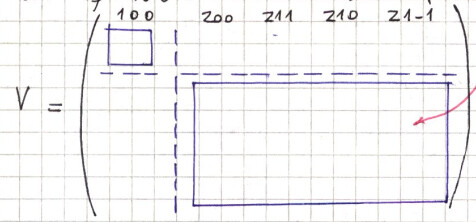
\includegraphics[width=0.5\textwidth]{images/fig_ft2_ejercicio7A.jpg}

Tenemos
\[
	\Braket{2 \ell m|-eEz|2\ell' m'} = -e E \Braket{2\ell m|z|2\ell' m'}
\]
y como el operador paridad cumple $\Pi z \Pi^{-1} = -z$ se da
\[
	\Pi \Ket{n\ell m} = (-1)^\ell \Ket{n\ell m}
\]
lo cual no es otra cosa que usar reglas de selección. Luego,
\[
	\Braket{2\ell m|-z|2\ell' m'} = (-1)^{\ell+\ell'} \Braket{2\ell m|z|2\ell' m'}
\]
y si $\ell+\ell'=L$ entonces el braket es nulo y sobreviven $\ell\neq \ell'$ de modo que
$\Braket{21m|z|200}$ es el que permanece.

Por Wigner-Eckart $z=T_0^1$ de modo que
\[
	\Braket{\a' j' m'|T_q^k|\a j m} = И \Braket{j k m q|j k j' m'}
\]
donde $И$ es una constante. Entonces
\[
	\Braket{21m|T_0^1|200} = И \Braket{0100 | 011m }
\]
desde lo cual sobreviven $\Braket{0100|011m}$ si $m=0$.

Entonces se tiene lo que ilustra la imagen

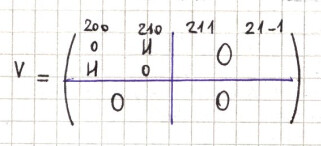
\includegraphics[width=0.5\textwidth]{images/fig_ft2_ejercicio7B.jpg}

y como es una matriz de Pauli su diagonalización es un juego de niños. Se tienen
\[
	\Ket{v_1} = \frac{1}{\sqrt{2}} \left( \Ket{200} + \Ket{210} \right)
	\qquad \qquad 
	\Ket{v_2} = \frac{1}{\sqrt{2}} \left( \Ket{200} - \Ket{210} \right)
\]

Si se cambia de base y se escribe el potencial $V$ en la base $\{ \Ket{100}, \Ket{v_1}, 
\Ket{v_2}, \Ket{211}, \Ket{21-1} \}$ se tiene

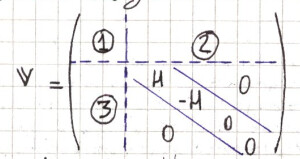
\includegraphics[width=0.5\textwidth]{images/fig_ft2_ejercicio7C.jpg}

que es una matriz diagonal por bloques. 
 
\end{ejemplo}

\subsection{Scattering a orden dos y OFPT}

Continuando con el orden dos de scattering por un $V\neq V(t)$ se tiene:
\[
	\omega_{i\to n}^{(2)} = \frac{2\pi}{\hbar}\left. \left| \overline{ V_{ni} + \sum_{m\neq i} 
	\frac{V_{nm}V_{mi}}{(E_i-E_m)}} \right|^2 \rho(E_n) \right|_{E_n\sim E_i}
\]

Para obtener los siguientes términos dentro del $\bar{||^2}$ podemos emplear un ardid gráfico conocido como 
{\it Old Fashioned Perturbation Theory}

\begin{figure}[!thb]
	\begin{center}
	\includegraphics[width=1.0\textwidth]{images/teo2_24.pdf}
	\end{center}
	\caption{}
\end{figure} 


Fíjese que en los estados intermedios estados virtuales $\Ket{m},\Ket{j}$ no se conserva la energía. Son 
propagadores.


\subsection{Perturbación armónica}

Sea un potencial armónico y hermítico 
\[
	V(t) = \mathbb{V} \euler^{i\omega t} + \mathbb{V}^\dagger \euler^{-i\omega t},
		\qquad \mathbb{V}\neq \mathbb{V}(t)
\]
quiero ver probabilidad de transición a orden uno,
\[
	C_n(t)^1 = -\frac{i}{\hbar} \int_0^t ( V_{ni}\euler^{i\omega t'}+ V_{ni}^\dagger \euler^{-i\omega t'} )
		\euler^{i\omega_{ni}t'}dt'
\]
\[
	C_n(t)^1 = -\frac{i}{\hbar} \left[ V_{ni} \int_0^t \euler^{i(\omega +\omega_{ni})t'} dt' + 
		V_{ni}^\dagger \int_0^t \euler^{i(-\omega +\omega_{ni})t'} dt' \right]
\]
\[
	C_n(t)^1 = -\frac{i}{\hbar} \left[ V_{ni} \frac{\euler^{i(\omega +\omega_{ni})t} -1}{i( \omega +\omega_{ni} )}
		+ V_{ni}^\dagger \frac{\euler^{i(-\omega +\omega_{ni})t} - 1}{i(-\omega +\omega_{ni})} \right]
\]
\[
	C_n(t)^1 = \frac{V_{ni}}{\hbar} \frac{1-\euler^{i(\omega +\omega_{ni})t}}{( \omega +\omega_{ni} )}
		+ \frac{V_{ni}^\dagger}{\hbar} \frac{1-\euler^{i(-\omega +\omega_{ni})t}}{(-\omega +\omega_{ni})}
\]
\[
	\lim_{t\to\infty} C_n(t)^1 = \frac{1}{\hbar}\left[ V_{ni}\delta(\omega_{ni}+\omega) 
		+ V_{ni}^\dagger \delta(\omega_{ni}-\omega) \right]
\]

Luego será nulo sólo si 
\[
	\omega_{ni} = -\omega \qquad \longrightarrow \qquad 
		\frac{E_n - E_i}{\hbar} = -\omega \quad E_n = E_i - \hbar\omega
\]
\[
	\omega_{ni} = -\omega \qquad \longrightarrow \qquad 
		\frac{E_n - E_i}{\hbar} = \omega \quad E_n = E_i + \hbar\omega
\]

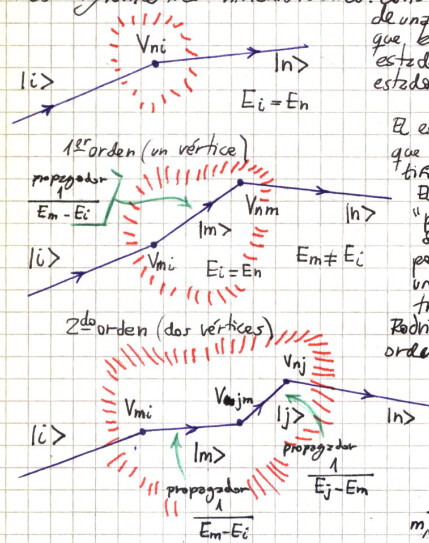
\includegraphics[width=0.6\textwidth]{images/fig_ft2_tre_ordenes_perturbativos.jpg}

\begin{figure}[htb]
	\begin{center}
	\includegraphics[width=1.0\textwidth]{images/teo2_25.pdf}
	\end{center}
	\caption{}
\end{figure} 

Luego,
\[
	\lim_{t\to\infty} C_n(t)^1
\]
representa la probababilidad de emitir o absorber fotones en una interacción. Se puede asociar que $V$ crea 
fotones y $V^\dagger$ destruye fotones. Para un átomo se tiene 
\begin{figure}[htb]
	\begin{center}
	\includegraphics[width=1.0\textwidth]{images/teo2_26.pdf}
	\end{center}
	\caption{}
\end{figure} 


Acá la sucesión de pictures como están en la carpeta:

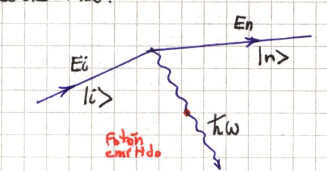
\includegraphics[width=0.4\textwidth]{images/fig_ft2_perturbativos_1a.jpg}
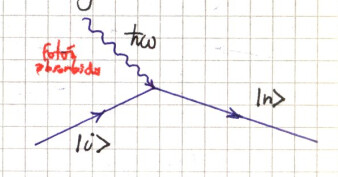
\includegraphics[width=0.4\textwidth]{images/fig_ft2_perturbativos_1b.jpg}

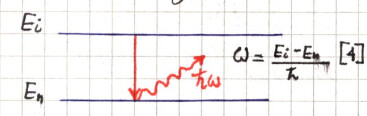
\includegraphics[width=0.4\textwidth]{images/fig_ft2_perturbativos_2a.jpg}
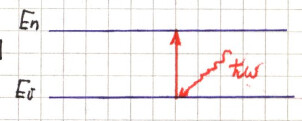
\includegraphics[width=0.4\textwidth]{images/fig_ft2_perturbativos_2b.jpg}

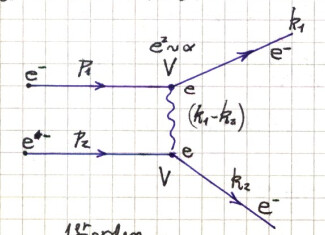
\includegraphics[width=0.4\textwidth]{images/fig_ft2_perturbativos_3a.jpg}
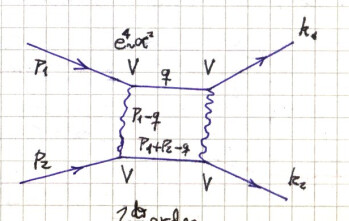
\includegraphics[width=0.4\textwidth]{images/fig_ft2_perturbativos_3b.jpg}



\section{Despoblamiento de estados iniciales}

Queremos ver con cual $v$ se despoblan los $\Ket{i}$. Para elllo me construyo un potencial {\it suave}
\[
	\lim_{\eta\to 0} V(t) = \euler^{\eta t} \mathbb{V}, \qquad  \mathbb{V} \text{cte.}
\]
donde $\eta$ es un parámetro regularizador.

Previa a la picture del desdoblamiento de estados iniciales estaban estas

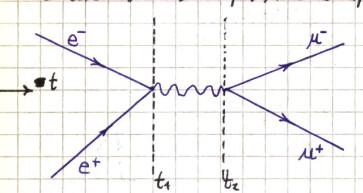
\includegraphics[width=0.4\textwidth]{images/fig_ft2_desdoblamiento_1a.jpg}
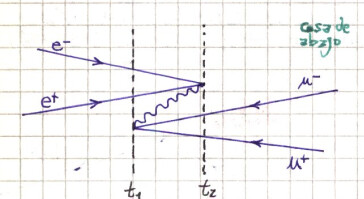
\includegraphics[width=0.4\textwidth]{images/fig_ft2_desdoblamiento_1b.jpg}

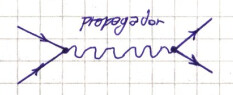
\includegraphics[width=0.4\textwidth]{images/fig_ft2_desdoblamiento_2a.jpg}
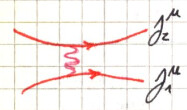
\includegraphics[width=0.4\textwidth]{images/fig_ft2_desdoblamiento_2b.jpg}

\begin{figure}[htb]
	\begin{center}
	\includegraphics[width=0.5\textwidth]{images/teo2_27.pdf}
	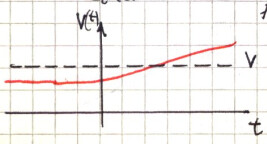
\includegraphics[width=0.4\textwidth]{images/fig_ft2_desdoblamiento_3.jpg}
	\end{center}
	\caption{}
\end{figure} 
\[
	C_n(t)^1 = \lim_{t\to\infty} -\frac{i}{\hbar} 
		\int_{t_0}^t V_{ni} \euler^{\eta t'} \euler^{i\omega_{ni} t'} dt'
\]
\[
	C_n(t)^1 = -\frac{i}{\hbar} V_{ni} \frac{\euler^{\eta t} \euler^{i\omega_{ni} t} }{\eta+i\omega_{ni}}
	\qquad \qquad 
 	|C_n(t)^1|^2 = \frac{|V_{ni}|^2}{\hbar^2} \frac{\euler^{2\eta t} }{\eta^2 + \omega_{ni}^2 }
\]
\[
	\dtot{}{t}|C_n(t)^1|^2 = 2 \eta \frac{|V_{ni}|^2}{\hbar^2} \frac{\euler^{2\eta t} }{\eta^2 + \omega_{ni}^2 }
\]
y tomando el límite $\eta \to 0$ 
\[
	\lim_{\eta\to 0} \dtot{}{t}|C_n(t)^1|^2 = 2 \frac{|V_{ni}|^2}{\hbar^2} 
			\frac{\eta }{\eta^2 + \omega_{ni}^2 } = \begin{cases}
	                    0 \quad \text{si}\;\; \omega_{ni}^2 \neq 0 \\
	                    \infty \quad \text{si}\;\; \omega_{ni}^2 = 0
	                   \end{cases}
\]
y llegamos a la regla de oro de Fermi,
\[
	\dtot{}{t}|C_n(t)^1|^2 = 2 \frac{|V_{ni}|^2}{\hbar^2} \delta(\omega_{ni}) \pi
\]

\subsection{Scattering sección eficaz}

$\Ket{k},\Ket{k}'$ son autoestados de momento (partículas libres),
\[
	|\vb{k}| = |\vb{k}'| 
\]
se conserva la energía. Consideraremos la aproximación más baja (aproximación de Born).
\begin{figure}[htb]
	\begin{center}
	\includegraphics[width=0.5\textwidth]{images/teo2_28.pdf}
	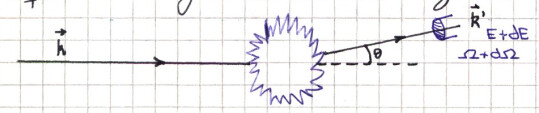
\includegraphics[width=0.5\textwidth]{images/fig_ft2_scattering_section.jpg}
	\end{center}
	\caption{}
\end{figure} 

\[
	\omega = \int \frac{2\pi}{\hbar}  \delta(E'-E) |\Braket{\vb{k}'|V|\vb{k}}|^2 \rho(E') dE'
\]
queremos calcular la densidad de estados de energía entre $(E,E+dE)$. Pensamos en una partícula libre en una 
caja $1D$ de longitud $L$.
\[
	N \euler^{i k_x x /\hbar}, \qquad \text{con} \;\; k_x = \frac{2\pi}{L}n_x
\]
pidiendo normalización unitaria $\Braket{k|k}=1$ se tiene 
\[
	\frac{1}{\sqrt{L}} \euler^{i k_x x /\hbar}
\]
con $L\to\pm\infty$ son $n_x,k_x$ continuas.
\[
	dk_x = \frac{2\pi}{L} dn_x \quad \longrightarrow \quad  dn_x = \frac{L}{2\pi} dk_x 
\]
\[
	E = \frac{\hbar^2k^2}{2m} = \frac{\hbar^2}{2m} \left( \frac{2\pi}{L}\right)^2 n^2 \quad 
	\longrightarrow \quad n^2 = \frac{L^2}{(2\pi)^2}k^2
\]
\[
	dE = \frac{\hbar^2}{m} k dk \quad \longrightarrow \quad dn = \frac{L}{2\pi}\frac{m}{\hbar^2 k} dE
\]
\[
	n^2 dn d\Omega = \left( \frac{L}{2\pi} \right)^3 \frac{mk}{\hbar^2} \:dE \:d\Omega
\]
donde $n^2\:dn\:d\Omega$ es la densidad de estados de energía $(E,E+dE)$ en $d\Omega$
\[
	n^2 \: dn \: d\Omega = \rho(E') dE'
\]

Con esto sale la integral obteniéndose
\[
	\omega_{\vb{k}-\vb{k}'} = 
	\frac{L^3}{(2\pi)^2} \frac{m}{\hbar^3} \left|\Braket{\vb{k}'|V|\vb{k}}\right|^2 k'd\Omega
\]

Esta es la probabilidad de transición entre los impulsos $\vb{k}$, $\vb{k}'$. Es el número de partículas en 
la unidad de tiempo por unidad de área 
\[
	\text{seccion eficaz} \equiv \dtot{\sigma}{\Omega}d\Omega =
	\frac{\text{\# de part en $d\Omega$ en la unidad de t}}
	{\text{\# de part incidentes en la unidad de t por unidad de área}}
\]

Un elemento de matriz $\Braket{k'|V|k}$ será 
\[
	\Braket{\vb{k}'|V|\vb{k}} = \int dx'\Braket{\vb{k}'|\vb{x}'} \Braket{\vb{x}'|V|\vb{k}} =
	\int d\vb{x}' \frac{1}{L^3} \euler^{i (\vb{k}-\vb{k}')\cdot \vb{x}} \; V(\vb{x}'),
\]
\begin{figure}[htb]
	\begin{center}
	\includegraphics[width=0.5\textwidth]{images/teo2_31.pdf}
	\end{center}
	\caption{}
\end{figure} 
la transformada de Fourier del potencial es, amén de constantes, la amplitud a primer orden 
\[
	|\vb{k} - \vb{k}'| = 2k\sin(\theta/2) \qquad \text{con} \; k=k' 
\]
Entonces para cualquier potencial esféricamente simétrico se puede hacer la integral 
\[
	\dtot{\sigma}{\Omega} =
	\left|\left( \frac{2m}{4\pi\hbar}\right)^2 \int d^3x'\;V(x)\euler^{i(\vb{x}-\vb{x}')\cdot\vb{x}'}\right|^2
\]
y expresamos todo en función de $q=q(\theta)$
\[
	\dtot{\sigma}{\Omega} =
	\left| -\frac{2m}{\hbar^2} \frac{1}{q} \int_0^\infty rV(r)\sin(q) dr \right|^2
\]

Utilizando un potencial de Yukawa primero y tomando el límite para llegar al de Coulomb tenemos la sección 
eficaz de Rutherford 
\[
	\dtot{\sigma}{\Omega} = \frac{2m^2e^4}{\hbar^4}\frac{1}{16k^4\sin^4(\theta/2)}
\]

hay que tomar el potencial de Yukawa y luego el límite porque el de Coulomb diverge de entrada

	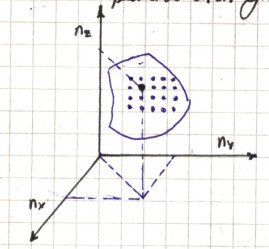
\includegraphics[width=0.5\textwidth]{images/fig_ft2_scattering_section_2.jpg}
	
	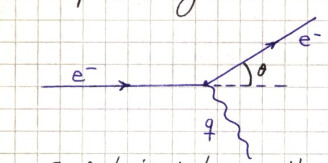
\includegraphics[width=0.5\textwidth]{images/fig_ft2_scattering_section_3.jpg}
		
	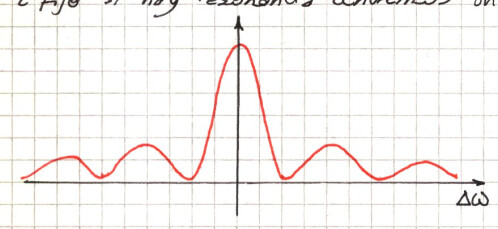
\includegraphics[width=0.5\textwidth]{images/fig_ft2_scattering_section_p1.jpg}
	
	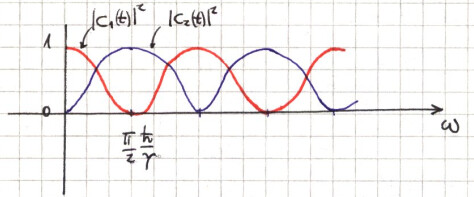
\includegraphics[width=0.5\textwidth]{images/fig_ft2_scattering_section_p2.jpg}
	
	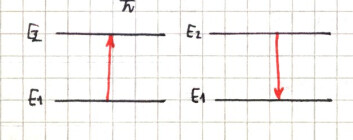
\includegraphics[width=0.5\textwidth]{images/fig_ft2_scattering_section_p3.jpg}



% \bibliographystyle{CBFT-apa-good}	% (uses file "apa-good.bst")
% \bibliography{CBFT.Referencias} % La base de datos bibliográfica

\end{document}
